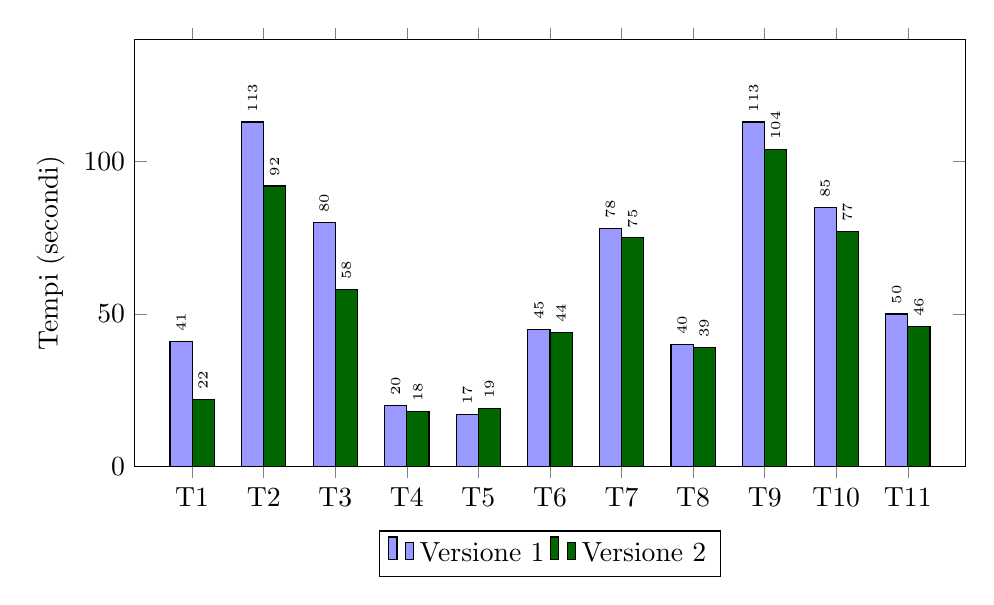
\begin{tikzpicture}
    \begin{axis}[
        ybar=0pt,
        bar width=8pt,
        enlarge x limits=0.08,
        legend style={at={(0.5,-0.15)}, anchor=north, legend columns=-1},
        ylabel={Tempi (secondi)},
        symbolic x coords={T1, T2, T3, T4, T5, T6, T7, T8, T9, T10, T11},
        xtick=data,
        nodes near coords,
        nodes near coords align={vertical},
        every node near coord/.append style={font=\tiny, rotate=90, anchor=west},
        width=\textwidth,
        height=7cm,
        ymin=0,
        ymax=140
    ]
        \addplot[fill=blue!40] coordinates { (T1,41) (T2,113) (T3,80) (T4,20) (T5,17) (T6,45) (T7,78) (T8,40) (T9,113) (T10,85) (T11,50) };
        \addplot[fill=green!40!black] coordinates { (T1,22) (T2,92) (T3,58) (T4,18) (T5,19) (T6,44) (T7,75) (T8,39) (T9,104) (T10,77) (T11,46) };
        \legend{Versione 1, Versione 2}
    \end{axis}
\end{tikzpicture}